\documentclass[12pt, a4paper]{article}
% --- Packages ---
\usepackage[utf8]{inputenc}
\usepackage[T1]{fontenc}
\usepackage[french]{babel}
\usepackage{graphicx} % Make sure this is here for images
\usepackage{booktabs}
\usepackage{amsmath}
\usepackage{geometry}
\usepackage{array}
\usepackage{enumitem}
\usepackage{hyperref}
\usepackage{xcolor}
\usepackage{titlesec}
\usepackage{lmodern}
\usepackage{microtype}
\usepackage{fancyhdr}
\usepackage{listings} % Added for code/JSON display
\usepackage[scaled=0.85]{beramono} % Added for a nicer monospaced font

% --- Font Configuration ---
% --- Color Definitions ---
\definecolor{primary}{RGB}{0,51,102}
\definecolor{secondary}{RGB}{102,102,153}
\definecolor{accent}{RGB}{204,0,0}
\definecolor{codegray}{rgb}{0.5,0.5,0.5}
\definecolor{codepurple}{rgb}{0.58,0,0.82}
\definecolor{codeblue}{rgb}{0,0,0.9}
\definecolor{codegreen}{rgb}{0.1,0.6,0.1} % Darker green for comments

% --- Page Geometry ---
\geometry{
  a4paper,
  left=2.5cm,
  right=2.5cm,
  top=2.5cm,
  bottom=2.5cm,
  headheight=15pt
}
% --- Header/Footer Setup ---
\pagestyle{fancy}
\fancyhf{}
\fancyhead[L]{\small Rapport de Stage - Semaine 3 - Jour 2} % Updated
\fancyhead[R]{\small Zakaria el Khaldi}
\fancyfoot[C]{\thepage}
\renewcommand{\headrulewidth}{0.4pt}
\renewcommand{\footrulewidth}{0.4pt}
% --- Title Formatting ---
\titleformat{\section}
  {\normalfont\Large\bfseries\color{primary}}
  {\thesection}{1em}{}
\titleformat{\subsection}
  {\normalfont\large\bfseries\color{secondary}}
  {\thesubsection}{1em}{}
\titleformat{\subsubsection}
  {\normalfont\normalsize\bfseries\color{accent}}
  {\thesubsubsection}{1em}{}
% --- List Formatting ---
\setlist[itemize]{leftmargin=*, nosep}
\setlist[enumerate]{leftmargin=*, nosep}
% --- Hyperlink Setup ---
\hypersetup{
  colorlinks=true,
  linkcolor=primary,
  urlcolor=secondary,
  citecolor=accent
}

% --- Listings Setup for JSON ---
\lstdefinestyle{json}{
    language=json,
    basicstyle=\ttfamily\footnotesize,
    numbers=left,
    numberstyle=\tiny\color{codegray},
    stepnumber=1,
    numbersep=5pt,
    backgroundcolor=\color{white!95!black}, % Very light gray background
    showspaces=false,
    showstringspaces=false,
    showtabs=false,
    frame=tb, % Top and bottom frame
    framextopmargin=3pt,
    framexbottommargin=3pt,
    rulecolor=\color{black!30!white},
    tabsize=2,
    captionpos=b,
    breaklines=true,
    breakatwhitespace=false,
    stringstyle=\color{codepurple},
    commentstyle=\color{codegreen},
    keywordstyle=\color{codeblue}, % For true, false, null
    morestring=[b]",
    literate=
     *{0}{{{\color{codeblue}0}}}{1}
      {1}{{{\color{codeblue}1}}}{1}
      {2}{{{\color{codeblue}2}}}{1}
      {3}{{{\color{codeblue}3}}}{1}
      {4}{{{\color{codeblue}4}}}{1}
      {5}{{{\color{codeblue}5}}}{1}
      {6}{{{\color{codeblue}6}}}{1}
      {7}{{{\color{codeblue}7}}}{1}
      {8}{{{\color{codeblue}8}}}{1}
      {9}{{{\color{codeblue}9}}}{1}
      {:}{{{\color{black}:}}}{1}
      {\{}{{{\color{black}{\{}}}}{1}
      {\}}{{{\color{black}{\}}}}}{1}
      {[}{{{\color{black}{[}}}}{1}
      {]}{{{\color{black}{]}}}}{1}
      {,}{{{\color{black}{,}}}}{1},
}


% --- Title Page Information ---
\title{\Huge\bfseries\color{primary} Rapport de Stage \\ 
      \Large Semaine 3 - Jour 2 : Expérimentation et Affichage Dynamique des Données} % Updated title
\author{\Large Zakaria el Khaldi}
\date{\large Le 21 mai 2025} % Updated date for Day 2 (assuming Day 1 was May 20th)

% --- Document Start ---
\begin{document}
% --- Cover Page ---
\begin{titlepage}
  \centering
  \vspace*{\stretch{0.5}}
  {\Huge\bfseries\color{primary} Rapport de Stage \par}
  \vspace{1cm}
  {\Large\itshape Semaine 3 - Jour 2 : Expérimentation et Affichage Dynamique des Données\par} % Updated title
  \vspace{2cm}
  
  \vspace{2cm}
  {\Large Zakaria el Khaldi\par}
  \vfill
  {\large Le 20 mai 2025\par} % Updated date of report submission / activity day
  \vspace*{\stretch{1}}
\end{titlepage}

% --- Table of Contents ---
\tableofcontents
\thispagestyle{empty}
\newpage

% --- Introduction ---
\section{Introduction}
\thispagestyle{fancy}
Ce rapport quotidien décrit les activités menées lors du deuxième jour de la troisième semaine de stage. Après la mise en place de la base de données MongoDB sur Atlas et l'établissement de la connexion avec l'application la veille, cette journée a été dédiée à l'expérimentation de la récupération des données et à leur affichage dynamique sur l'interface utilisateur. De plus, une réflexion a été entamée concernant les limitations potentielles de la solution de base de données actuelle, menant à la planification d'explorations technologiques alternatives.

% --- Day's Accomplishments ---
\section{Activités du Jour (Mardi 20 Mai 2025)} % Updated day and date

\subsection{Expérimentation avec les Requêtes MongoDB pour la Récupération de Données}
La journée a débuté par une phase d'expérimentation intensive avec les requêtes MongoDB. Différentes approches pour interroger la base de données Atlas ont été testées afin d'identifier les méthodes les plus performantes et adaptées pour récupérer les métadonnées des cours et tutoriels.

\subsection{Développement de la Logique d'Extraction des Métadonnées Frontend}
Une fois les requêtes optimisées, l'étape suivante a consisté à implémenter la logique applicative pour récupérer les informations essentielles telles que le langage de programmation, le niveau de difficulté des cours (par exemple, "Beginner", "Intermediate"), et le nombre de tutoriels disponibles pour chaque cours.

\subsection{Affichage Dynamique des Cours sur l'Interface Utilisateur}
Les données récupérées ont ensuite été utilisées pour alimenter dynamiquement l'interface utilisateur. Les cours, avec leurs métadonnées (difficulté, nombre de tutoriels), sont désormais affichés sous forme de cartes interactives dans la section gratuite du site, comme illustré à la Figure \ref{fig:dynamic_course_cards}. Cette étape concrétise la connexion entre le backend et le frontend pour la présentation du contenu.

\begin{figure}[htbp]
  \centering
  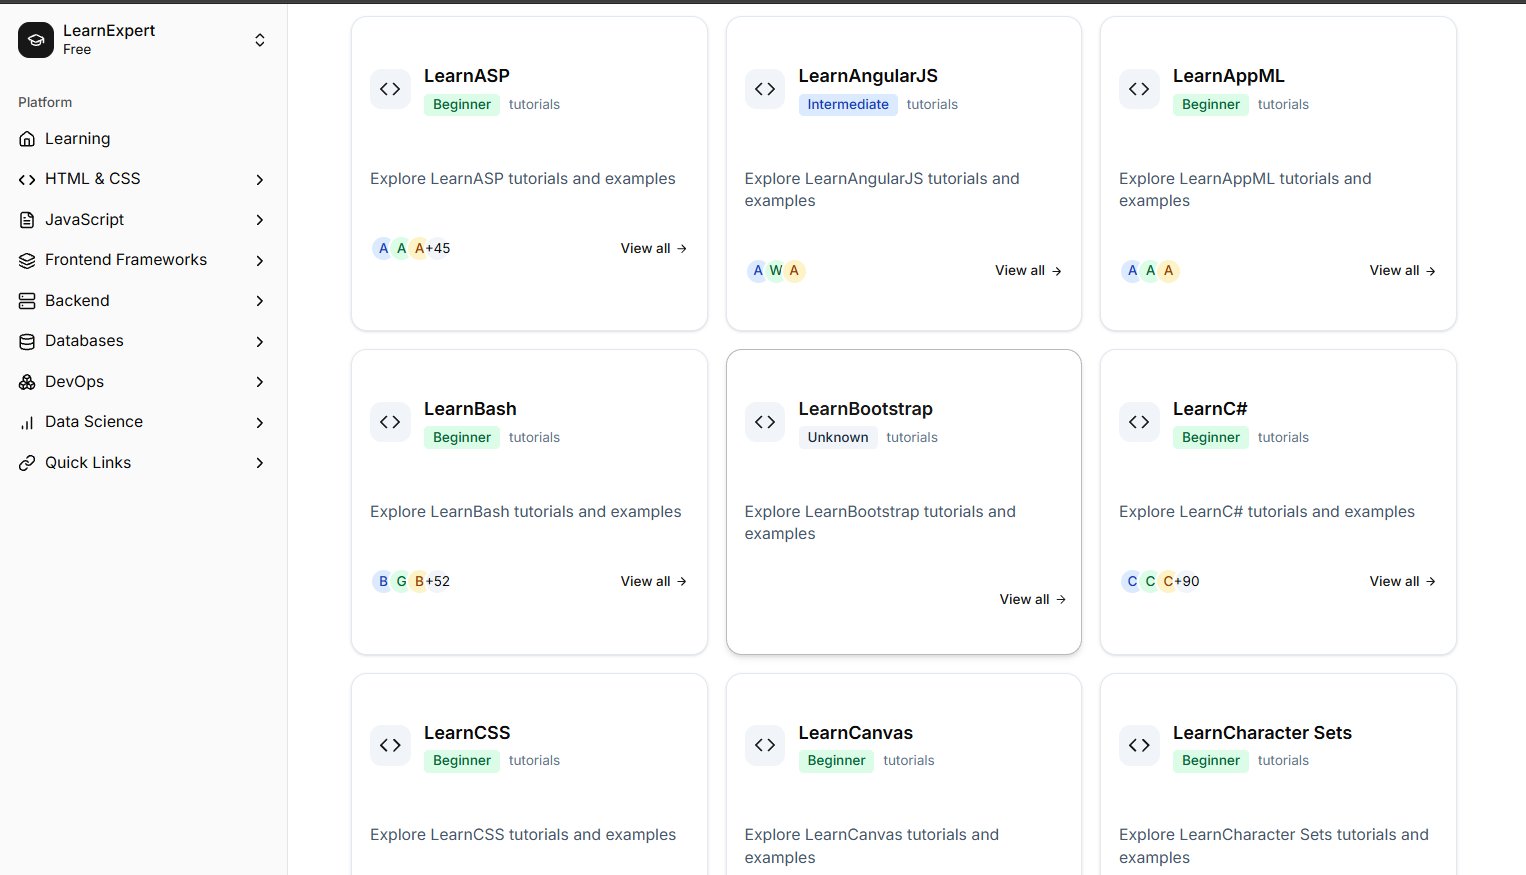
\includegraphics[width=0.9\textwidth]{Screenshot 2025-05-20 164411.png} % Replaced with the new image
  \caption{Affichage dynamique des listes de cours et tutoriels sous forme de cartes.} % Updated caption
  \label{fig:dynamic_course_cards} % Updated label
\end{figure}

\subsection{Analyse des Limitations de MongoDB Atlas et Planification d'Alternatives}
Au cours de l'intégration, certaines limitations perçues de MongoDB Atlas (\url{https://cloud.mongodb.com}) dans le contexte spécifique du projet ont été identifiées. Cela a conduit à la décision d'explorer d'autres fournisseurs de bases de données cloud ainsi que d'autres types de bases de données, notamment PostgreSQL avec son support JSON, afin de s'assurer que la technologie choisie est la plus adaptée aux besoins à long terme du projet.

\subsection{Planification pour Demain (Mercredi 21 Mai 2025)} % Updated day and date
La journée de demain sera consacrée à l'exploration technologique et à la consolidation des choix d'infrastructure de données :
\begin{itemize}
  \item Suspendre temporairement l'intégration de nouvelles fonctionnalités frontend pour se concentrer sur l'infrastructure de données.
  \item Mener une étude comparative et expérimenter avec d'autres fournisseurs de services de base de données cloud.
  \item Évaluer PostgreSQL, en particulier ses capacités de gestion de données JSON, comme alternative potentielle à MongoDB, pour voir ce qui est le mieux adapté aux besoins du projet.
  \item En fonction des résultats de ces expérimentations, prendre une décision éclairée sur la technologie de base de données à utiliser.
  \item Une fois la technologie de base de données choisie et validée, l'intégration du contenu dynamique reprendra, en commençant par l'implémentation du chargement paresseux (lazy loading) des cartes de cours pour améliorer les performances.
\end{itemize}

\section{Conclusion}
Cette deuxième journée de la troisième semaine a été productive, avec la mise en place réussie de l'affichage dynamique du contenu des cours. Plus important encore, elle a initié une phase cruciale de réflexion stratégique sur les choix technologiques de la base de données. L'expérimentation planifiée pour demain vise à s'assurer que le projet repose sur une fondation de données robuste, scalable et adaptée, avant de poursuivre l'intégration de fonctionnalités plus avancées et d'optimisations telles que le lazy loading.

\end{document}